\documentclass[final,los,index,glossary,loa]{ryethesis}
\usepackage{amsmath}
\usepackage{amsfonts}
\usepackage{amsthm}
%
% Note that this usage example is not an introduction to using LaTeX. You are highly recommended to check out Leslie Lamport's "LaTeX: A Document Preparation System". Please read through this file to get started using the ryethesis document class, including all comments!
%
% This sample includes packages which are part of the current TeX Live distribution. The TeX Live 
% distribution is the easiest way to get up and running with TeX. See http://tug.org/texlive

% Available options to ryethesis class:
% draft - Produce a one-sided, double-spaced draft (figures replaced by placeholders).
% review - Produce a one-sided, 1.5-spaced version for review by examiners.
% final (default) - Produce a two-sided, 1.5-spaced final version
% lof (default) | nolof - Enable | disable a list of figures
% lop | nolop (default) - Enable | disable a list of plates
% loi | noloi (default) - Enable | disable a list of illustrations
% lot (default) | nolot - Enable | disable a list of tables
% loa (default) | noloa - Enable | disable a list of appendices (separate from TOC)
% los | nolos (default) - Enable | disable a list of symbols (nomenclature)
% glossary | noglossary (default) - Enable | disable a glossary of terms
% index | noindex (default) - Enable | disable an index
% nohyperref - Disable the loading of hyperref

% List of Symbols / Nomenclature
%=====================
% Note that current SGS policy does not specify a requirement for a nomenclature list. In keeping with the "List of ..." model, the nomenclature is presented as a "List of Symbols". The List of Symbols currently appears as the last item in the front matter. 
%
% The nomenclature must be processed using the 'makeindex' command, similar to the creation of an index. For example:
%   makeindex ryesample.nlo -s nomencl.ist -o ryesample.nls 
%
% Symbols can be defined with the \nomenclature command in the body of the text (see below for examples).

% Some of the class options can be toggled in the preamble. The following commands are available (function should be obvious by name):
%  \includelistoftables
%  \nolistoftables
%  \includelistoffigures
%  \nolistoffigures
%  \includelistofplates
%  \nolistofplates
%  \includelistofillustrations
%  \nolistofillustrations
%  \includelistofappendices
%  \nolistofappendices
%  \includenomenclature
%  \nonomenclature
%  \includeglossary
%  \noglossary
%  \includeindex
%  \noindex

% If you wish to include pictures, I recommend the graphics package. This is not
% loaded by the ryethesis class. 
\usepackage{color}
\usepackage{graphicx}

% Add any other packages you wish to load here in the preamble. 
% \usepackage{somecoolpackage}

% This sample uses a modified version of the Chicago Manual of Style bibtex style, 
% which requires the inclusion of chicago.sty. 
%\usepackage{chicago}

% In the pre-amble, define some of necessary information for the document frontmatter.

% Specify the author (required):
% \author{Your Full Name} 
\author{Adolphus Egerton Ryerson}

% Specify the title of the document (required):
% \title{The Title of Your Thesis or Dissertation} 
\title{De Finibus Bonorum et Malorem}

% The document type can be specified with the following commands. Each document type will
% have a slightly different title page.
% \thesis - (default) Specify that the document type is a thesis
% \dissertation - Specify that this is a dissertation.
% \MRP - Specify that this is a masters research project (e.g. MEng project)

% Specify the type of degree (e.g. Masters of Applied Science, Doctor of Philosophy). Do not use
% abbreviations.
% \degreeName{Full Degree Name}  
\degreeName{Doctor of Philosophy}

% Specify the year of the degree:
% \degreeYear{####}
\degreeYear{1847}

% Specify the program:
% \program{Program Name}
\program{Education}

% Specify any previous degrees (A through D)
% \prevDegreeA{Degree Name}{University}{Year}
% \prevDegreeB{Degree Name}{University}{Year}
% \prevDegreeC{Degree Name}{University}{Year}
% \prevDegreeD{Degree Name}{University}{Year}
% Previous degrees will be listed with degree A first.
\prevDegreeA{Masters of Education}{Ryerson}{1845}
\prevDegreeB{Masters of Business Administration}{Ryerson}{1843}
\prevDegreeC{Masters of Something Else}{Ryerson}{1841}
\prevDegreeD{Bachelor of Arts}{Ryerson}{1839}

% If the degree is offered in partnership with another university, specify the university 
% with the \partnerUniversity command
% \partnerUniversity{Other University}
\partnerUniversity{Hogwarts University}

% Much of the front matter and back matter is automatically inserted in the correct location. 
% Use the following commands to insert the necessary content.

% The abstract. Current SGS requirement is the same as the UMI requirements: double-spaced, maximum 350 words for a PhD, 150 words otherwise. Use the \abstract command to specify the content of the abstract. The name, title, etc will be generated automatically.
%
% This abstract uses the optional acronyms defined in the glossary. The first occurance of a new
% acronym will be written out in full followed by the acronym in brackets. This feature is reset at the 
% beginning of the main body of the text.

\abstract{% A 350 word abstract. This will likely take 2 pages
\Gls{LI} dolor sit amet, consectetur adipiscing elit. Aliquam tempus ultrices dolor, quis convallis est tempor id. Nam semper rhoncus diam, nec dapibus est tristique sed. Praesent non ligula eu metus laoreet ultrices. Praesent sagittis accumsan nibh, in adipiscing dui pretium vel. Nunc justo quam, tincidunt non adipiscing eu, facilisis eu risus. Etiam vitae ipsum felis, non sodales massa. Cras volutpat ultrices dolor, in aliquet felis ullamcorper quis. Vivamus feugiat auctor diam. Curabitur lectus lorem, ultrices eget ultrices non, scelerisque quis diam. Integer eget neque sed diam vehicula consequat. Phasellus aliquam elementum velit, eget suscipit enim mattis sed. Sed consequat commodo condimentum. Sed orci eros, posuere vitae consectetur et, faucibus ultricies justo. Phasellus vitae magna justo.

Vestibulum ante ipsum primis in faucibus orci luctus et ultrices posuere cubilia Curae; Duis eget enim in magna sodales condimentum. Mauris aliquam dolor in risus aliquet pharetra. Ut accumsan faucibus dui vel vehicula. Sed justo diam, laoreet vel imperdiet sit amet, porta sit amet leo. Donec ac quam massa. Class aptent taciti sociosqu ad litora torquent per conubia nostra, per inceptos himenaeos. Nam convallis quam vel lorem viverra nec lacinia metus consectetur. Aliquam erat volutpat. Mauris consequat ullamcorper consectetur. Aenean urna risus, iaculis porta sodales at, egestas a odio. In sed ultricies dui. Sed tincidunt sem et lectus convallis nec posuere purus condimentum.

In purus ipsum, euismod ac dictum non, luctus ut ligula. Nullam neque elit, faucibus non elementum vitae, sodales ac turpis. Sed sit amet mauris at purus facilisis interdum. Nunc nisl eros, faucibus in viverra in, fringilla ac velit. Praesent nec quam sed augue adipiscing dictum in et nibh. Sed non lectus in mi ultrices rutrum ac non ligula. Etiam ac neque et sapien semper imperdiet ornare vitae felis. Etiam dignissim purus id sem ultrices malesuada. Phasellus ut leo nec quam semper blandit ac quis urna. Fusce egestas turpis at tortor imperdiet pretium. Nam id enim enim. Quisque felis metus, iaculis id pretium et, pharetra ac augue. Morbi tempus sollicitudin ligula a condimentum. Sed ultricies purus in eros laoreet mollis. Nullam tempus dolor sit amet lectus molestie aliquam. Morbi nisi diam, auctor.
}

% The acknowledgements. Similar to the abstract, specify the content of the acknowledgments section using the \acknowledgement command. Acknowledgements are optional. 

\acknowledgements{
Lorem ipsum dolor sit amet, consectetur adipiscing elit. Praesent non sem justo, ut laoreet lorem. Maecenas sit amet hendrerit risus. Vivamus vitae neque dolor. Curabitur ultrices nisi quis arcu dapibus interdum. Integer id nunc velit, eget egestas nisi. Aenean at metus eget arcu fermentum ullamcorper et vel mauris. In lacinia ultrices eros eu mollis. Fusce tincidunt quam non nunc tristique pulvinar. Duis quis justo elit, et adipiscing metus. Sed in faucibus magna. Nulla ut posuere diam. Morbi pharetra condimentum nunc, at consequat risus faucibus quis. Donec odio purus, eleifend vitae volutpat ac, lacinia non ligula. Class aptent taciti sociosqu ad.}

% The dedication. Similar to \acknowledgements command, the dedication is optional.
\dedication{
Lorem ipsum dolor sit amet, consectetur adipiscing elit. Integer pulvinar cursus dolor venenatis mollis. Quisque eleifend elementum varius. Nulla rhoncus eros neque, in rhoncus urna. Phasellus in purus et nisi hendrerit venenatis. In felis tortor, venenatis eu auctor nec, fermentum sed sem. Duis nisi tellus, mattis in accumsan sit amet.}

% Bibliography/References/End Notes
% The following commands should be used along with BibTeX input files. Use the \cite commands as needed throughout the main matter.
%
% Specify your desired BibTeX bibliographic style. 
% This sample includes a modified version of chicago.bst which includes URL support, created with the urlbst utility. You can enable it as follows but you will need to install the url package.
%\bibliographystyle{chicagourl}
% You are free to use what ever BibTeX style you wish. See the \bibliographystyle 
% command below.
\bibliographystyle{plain}
%
%
%
% The \bibliography command is inserted automatically in the correct place (ahead of any glossary but after the appendix). Use the \addtoreferences command to add BibTeX .bib files to the input list. Note that this is not the usual way of doing this in LaTeX but works to fit the bibliography in the correct place. You can divide your references among multiple BibTeX .bib files, and include each one with a \addtoreferences command.
%
% \addtoreferences{bibfilename} 
\addtoreferences{ryesample}
%
% The default heading for a reference list is "References". To use "Bibliography" instead, use the \usebibliography command
% \usebibliography
% or to use "End Notes" use the \useendnotes command.
% \useendnotes
%

% Glossaries are implemented using the `glossaries' package. Usage is optional but helpful for defining acronyms.

\newglossaryentry{Lorem}{name={lorem},description={lorem ipsem dolor sit amet}}
\newglossaryentry{Bonorum}{name={bonorum},description={Pellentesque tincidunt mauris id odio venenatis bibendum}}
\newglossaryentry{Malorem}{name={malorem},description={Nam vestibulum libero et molestie mollis}}
\newacronym{LI}{LI}{lorem ipsum}

% Everything after the \begin{document}, excluding any \appendix command is considered to be the main matter of the document.
%
\begin{document}
\chapter{Introduction}
\textit{Please note that this sample is not a beginner's introduction on using \LaTeX{}. While it's not difficult to get started with \LaTeX{}, especially if using the \href{http://tug.org/texlive}{\TeX{} Live} distribution, please see Leslie Lamport's ``LaTeX: A Document Preparation System'' as a starting point for learning \LaTeX{}.}

\textit{For the main matter of your thesis use the following sectional hierarchy: (part), chapter, section, subsection, paragraph, subparagraph. Each of these divisions can be indicated using the respective \LaTeX{} commands (e.g.\ \texttt{\textbackslash{chapter}} for a new chapter). Chapters will start on the right-hand page in two-sided mode with clear, empty pages inserted as needed in duplex mode. In draft mode, no empty pages will be inserted.}

\textit{This \LaTeX{} sample document includes additional comments regarding usage in the source.}

\section{Background}
\Gls{Lorem} ipsum dolor sit amet, consectetur adipiscing elit. Praesent eu mauris tortor. Aliquam erat volutpat. Morbi gravida varius ornare. Duis vitae erat a odio pretium pharetra ornare sit amet urna. Cum sociis natoque penatibus et magnis dis parturient montes, nascetur ridiculus mus. Nulla tempor lacinia augue, nec blandit lacus placerat nec. Phasellus non blandit dui. Donec lobortis eros id dolor semper consectetur. Mauris laoreet metus ut elit fringilla adipiscing posuere neque mattis. Aliquam turpis nibh, porta tristique elementum pellentesque, pharetra non neque. Cras dapibus ullamcorper dolor, ac tincidunt erat fermentum adipiscing. Fusce molestie, velit lobortis sollicitudin consectetur, ante metus tempus tortor, quis cursus lacus augue sit amet sem. Maecenas nibh urna, ullamcorper eget suscipit ac, fermentum ut ante.\footnote{Footnotes will be included on the same page whenever possible. Cras congue consectetur elit, ac lobortis tortor laoreet sit amet. Cras mauris est, feugiat vitae elementum eget, aliquam consequat urna. Aliquam ac vestibulum enim. Suspendisse.} Sed non lectus sapien. Suspendisse commodo sagittis massa, eget consectetur ipsum hendrerit sed. Sed condimentum tortor quis tortor facilisis aliquam. Ut tristique diam sit amet eros convallis ac eleifend felis imperdiet. Nam eros nunc, condimentum in blandit et, consectetur ac velit. Etiam sem purus, hendrerit id adipiscing et, viverra nec mi. Proin auctor, dolor at pretium facilisis, massa mauris blandit felis, ut vestibulum nibh purus non lectus.\footnote{Integer ornare vestibulum magna, in vestibulum lacus dapibus ac. Maecenas et enim et metus malesuada.}

% Attribution to references are done using BibTeX. 
Suspendisse suscipit urna quis lacus egestas interdum. \Gls{LI} dolor sit amet, consectetur adipiscing elit \cite{Ryerson:bio}. Cras libero lacus, facilisis sit amet tempus at, condimentum vitae urna. Nam sit amet tortor ut risus commodo tincidunt. Nam sit amet sodales est. Curabitur tempus neque vitae portor porta gravida \cite{Ryerson:v1,Ryerson:v2}
% Equations can be entered in the usual manner. The 'nomencl' package is loaded by the class by default. A nomenclature list can be created as well using the \nomenclature command with the 'nom' class option. To avoid odd spacing issues, use the \nomenclature command within an equation environment or as a separate paragraph. Do not embed within a paragraph. 
\begin{equation}
a^2+b^2=c^2
\nomenclature{a}{length of adjacent side}
\nomenclature{b}{length of opposite side}
\nomenclature{c}{length of hypotenuse}
\end{equation}
etiam dolor turpis, rhoncus nec adipiscing et, ullamcorper ut eros. Ut auctor pellentesque ante, ac ullamcorper lacus pharetra eu. In sodales euismod elementum. Phasellus urna erat, ornare ut vulputate vel, iaculis non elit. Vivamus faucibus ullamcorper consequat.

\begin{table}
\begin{center}
\begin{tabular}{|c|c|c|}\hline
& \gls{Bonorum} & \gls{Malorem} \\ \hline
Lorem & X & \\\hline
Ipsum &  & X \\\hline
\end{tabular}
\caption[Lorem ipsum dolor sit amet, consectetur adipiscing elit.]{\textit{Tables should be handled as floats using the \texttt{table} environment.} \Gls{LI} dolor sit amet, consectetur adipiscing elit. Duis nibh.}\label{tab::1}
\end{center}
\end{table}

\subsection{Bonorum}\index{Bonorum}
Pellentesque tincidunt mauris id odio venenatis bibendum. Etiam porta, tellus nec consectetur laoreet, nisl orci mattis nisl, at aliquam nunc ante quis leo. Aliquam facilisis lectus eu justo laoreet dictum. Ut aliquam magna arcu. Sed convallis, tellus non elementum consequat, tellus erat molestie dui, id mattis arcu nisl et mi. Praesent ac interdum nibh. Nunc sed mi diam, sed hendrerit dolor. Cras sed orci ut lacus rutrum consequat. Donec tincidunt blandit feugiat. Nulla aliquet consectetur bibendum.

Donec eget gravida ipsum. Vestibulum scelerisque sem eu purus varius bibendum. In fringilla cursus purus, et rutrum est porta sagittis. Quisque non massa ut velit lacinia aliquet ut non sapien. Duis accumsan viverra sem a condimentum. Pellentesque habitant morbi tristique senectus et netus et malesuada fames ac turpis egestas. Nam lobortis diam sed enim pharetra egestas. Quisque non urna risus. Duis sodales sapien mauris, iaculis sagittis libero. Quisque tellus nisl, ullamcorper quis vehicula id, convallis quis libero. Suspendisse nec sem velit, nec rhoncus ipsum. Aliquam a ante dui. Class aptent taciti sociosqu ad litora torquent per conubia nostra, per inceptos himenaeos. Vivamus pharetra dolor arcu. Nunc egestas est sit amet sapien sollicitudin elementum.

\subsection{Malorem}\index{Malorem}
Nam vestibulum (Fig.~\ref{fig::1}), libero et molestie mollis, urna est posuere arcu, et ornare nisi ligula nec est. Mauris volutpat turpis id purus gravida dictum. Nulla non justo eget elit vehicula tempus. Vivamus quis nibh leo. Nullam metus nulla, aliquam scelerisque sodales sed, porta nec lectus. Mauris iaculis dignissim lacus in bibendum. Maecenas vel massa ut orci dignissim placerat ut sed ante. Morbi luctus lacus dolor (Table~\ref{tab::1}). Aliquam luctus, arcu quis laoreet ultricies, risus ligula fermentum leo, tempus porttitor nibh libero nec justo. Aliquam erat volutpat. Aliquam sagittis placerat ligula, a aliquam justo vulputate in.
\begin{figure}
\begin{center}
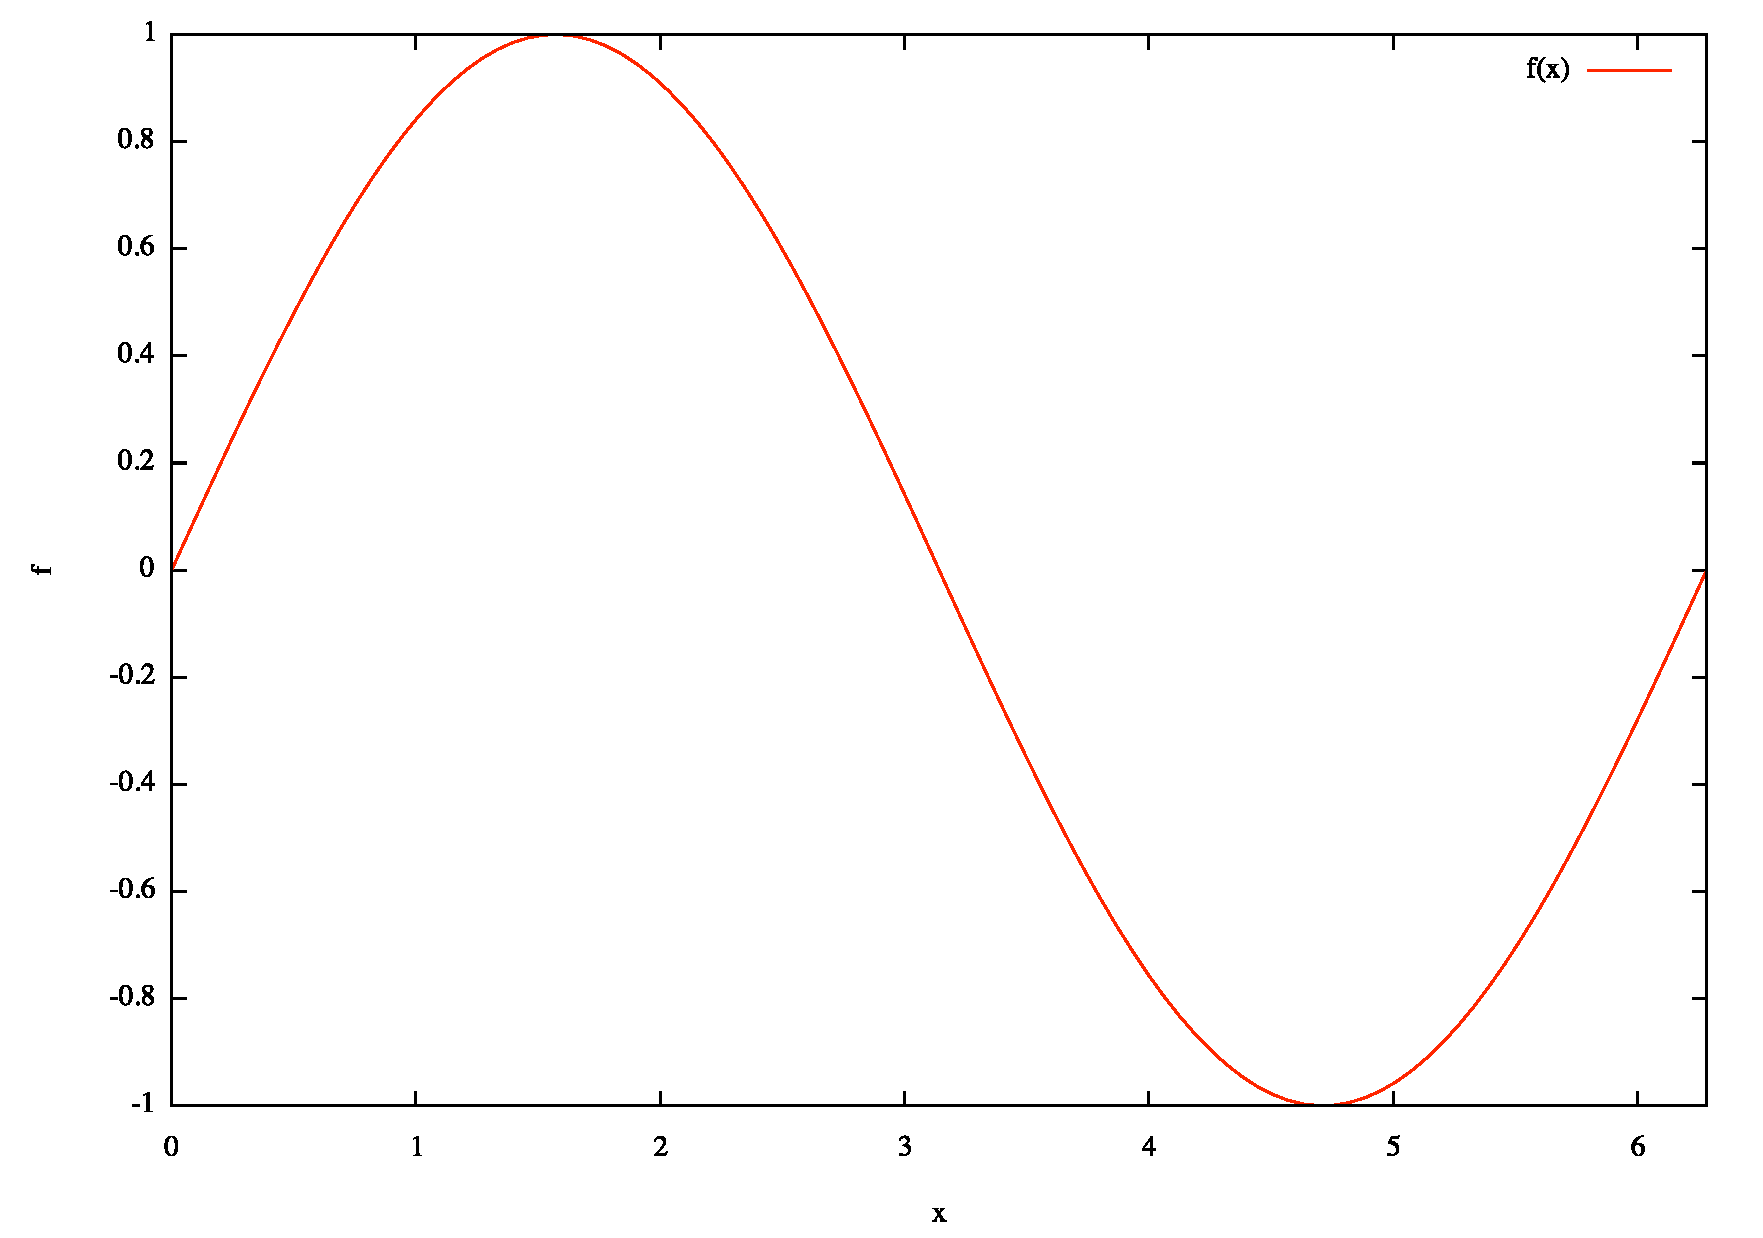
\includegraphics[width=\textwidth,keepaspectratio=true]{figure1.pdf}
\caption[Lorem ipsum dolor sit amet, consectetur adipiscing elit.]{\textit{Figures should be included using the \texttt{figure} float environment.} \Gls{LI} dolor sit amet, consectetur adipiscing elit. Duis nibh.}\label{fig::1}
\end{center}
\end{figure}
\chapter{Lorem}
\Gls{LI} dolor sit amet, consectetur adipiscing elit. Integer pretium aliquam elit ac sollicitudin. Curabitur sem urna, laoreet non fermentum id, rhoncus eget ante. Pellentesque habitant morbi tristique senectus et netus et malesuada fames ac turpis egestas. Mauris elementum ante non eros consequat luctus. Suspendisse lobortis accumsan tempus. Nullam ut dolor vestibulum erat tempor ornare bibendum vitae nisl. Praesent ornare odio molestie ligula iaculis ac eleifend ante dignissim. Vestibulum nec elit sed tortor sollicitudin euismod. Nulla facilisi. Sed nec fermentum nisi. Morbi et porta lectus. Praesent vel urna quis mi ornare pellentesque id quis ligula. Aliquam eu feugiat augue. Nunc faucibus nulla orci, et ornare leo. In vestibulum pellentesque mi vitae posuere.

\section{Sed Sed Elit}
Sed sed elit et tortor volutpat mollis. Donec vel placerat orci. Vivamus condimentum dictum gravida. Pellentesque eleifend blandit lorem, vitae lacinia sapien ultrices et. Morbi dignissim, elit sit amet facilisis sodales, mi diam accumsan libero, porttitor tincidunt diam lectus et mi. Proin sollicitudin massa sed sapien porta a semper sem fringilla. Quisque nec odio ac augue aliquam tristique. Quisque volutpat pulvinar nisi et tempor. Quisque in tellus quis mauris ultrices lacinia id eget lorem. Nunc placerat rutrum mauris, id sollicitudin neque tincidunt eu. Proin sed diam mauris. Proin varius quam nec dolor egestas quis tempus mauris dignissim. Ut a sem risus. Proin ultrices, turpis ut viverra convallis, nulla mauris interdum enim, vel tincidunt ipsum libero id orci. Nullam cursus neque eget nisi commodo sit amet volutpat purus semper. Praesent lacus ante, facilisis in suscipit ut, cursus tempus tellus.

Vestibulum ultrices vulputate justo, quis cursus lorem aliquet a. Cum sociis natoque penatibus et magnis dis parturient montes, nascetur ridiculus mus. Duis sagittis justo id ligula mollis varius a ut arcu. Morbi semper ante vitae leo rhoncus mattis. Suspendisse scelerisque feugiat dolor ut adipiscing. Maecenas et pretium diam. Aliquam dictum enim elit, a vehicula justo. Nullam euismod arcu in metus bibendum condimentum. Donec at nunc eu arcu semper iaculis ut at nisl. Donec nec libero in sem hendrerit porta. Aliquam vitae lorem vitae dui auctor lacinia. Vestibulum eu dolor ut turpis varius venenatis in quis augue.

\section{Etiam}
Etiam dictum auctor pharetra. Pellentesque quam leo, pretium sagittis vulputate a, lobortis et diam. Vestibulum rutrum massa et est porta luctus. In non risus ac magna posuere pulvinar. Morbi vitae libero vel erat blandit ultrices ac eget est. Suspendisse tellus turpis, sodales ut varius a, mattis eu massa. Donec ac purus eros. Integer vel varius justo. Sed suscipit sodales condimentum. Integer augue urna, euismod eget feugiat blandit, facilisis id lorem. \Gls{LI} dolor sit amet, consectetur adipiscing elit. Nulla eu lectus sem, ut tristique mauris. Maecenas tincidunt dui non ante lacinia et commodo massa adipiscing. Aenean hendrerit molestie tortor vitae malesuada. Nullam et scelerisque metus.

Pellentesque mollis accumsan nisi, vel tristique turpis luctus non. Fusce tristique blandit scelerisque. Praesent interdum aliquam felis ac feugiat. Integer accumsan ornare lacus, eget vehicula ante tincidunt eu. Pellentesque mauris diam, consequat ut pharetra sed, faucibus nec risus. Sed vulputate porttitor mauris, quis mollis dui egestas et. Etiam cursus adipiscing cursus. Integer rhoncus consequat dapibus. Sed interdum, odio non fringilla volutpat, ante arcu adipiscing dui, a pellentesque lorem risus a nisi. Phasellus nisi odio, dignissim a feugiat eu, fermentum eu odio. Ut augue ante, tristique eget aliquam a, mollis sed nisi.

% The back matter is inserted automatically in the correct SGS-required order, thus it is important that you define the content of the appendices within the \appendix command. This command can be defined in either the preamble or within the document environment. Use chapter and other section marks as normal. According to SGS policy, the appendices should appear in a List of Appendices instead of the regular Table of Contents. Note that figures, tables and other floats which appear in the appendix will be listed in the appropriate List of Figures, etc.

\appendix{
\chapter{Lorem Ipsum}
\textit{The appendices are part of the back matter, with chapters being enumerated with letters instead of numbers. Page numbering is continuous with the main matter. Note that SGS policy states that appendices be listed in the List of Appendices rather than the Table of Contents.}
\section{Lorem}
\Gls{LI} dolor sit amet, consectetur adipiscing elit. Maecenas nulla lorem, venenatis et suscipit eu, ullamcorper tempor purus. Maecenas aliquet vestibulum libero, eu tempor diam ullamcorper eu. Pellentesque vel urna id nibh tempus blandit a tristique dui. Nunc sodales feugiat risus, ac varius lacus adipiscing a. Duis pulvinar euismod viverra. Maecenas ullamcorper aliquet lorem pellentesque gravida. Vivamus tincidunt massa eu turpis ultricies ac placerat erat molestie. Phasellus nec tellus neque. Praesent nec dapibus dui. \Gls{LI} dolor sit amet, consectetur adipiscing elit. Donec nec erat vitae libero tristique varius nec volutpat est. Nullam viverra, mi a tristique commodo, ante erat tincidunt erat, at vestibulum ipsum tellus in diam. Sed imperdiet mauris vel eros aliquam pellentesque a aliquam ipsum. Duis eget leo nibh. Mauris justo nisl, dictum a tempor sit amet, semper et enim. Mauris augue nisi, mattis vel pretium id, convallis laoreet orci. Sed vestibulum nisi sit amet enim sagittis porttitor. Duis ut nunc vel magna convallis vehicula eu eu turpis. In hac habitasse platea dictumst. Aenean condimentum fermentum risus, viverra ultricies nisl dapibus id.

Donec arcu felis, vulputate fringilla vestibulum sed, interdum eu ipsum. Mauris egestas egestas libero, ut dictum enim tincidunt vel. Nunc sit amet arcu turpis, ac commodo ante. Aenean dictum urna urna, sed mattis tellus. Vivamus cursus condimentum ullamcorper. Nunc ut lorem enim. Morbi tempor vestibulum rhoncus. Phasellus nec neque urna. Aliquam sollicitudin scelerisque erat sit amet hendrerit. Quisque a libero felis. Pellentesque iaculis gravida massa nec tincidunt. Nulla facilisi.

\begin{figure}
\begin{center}
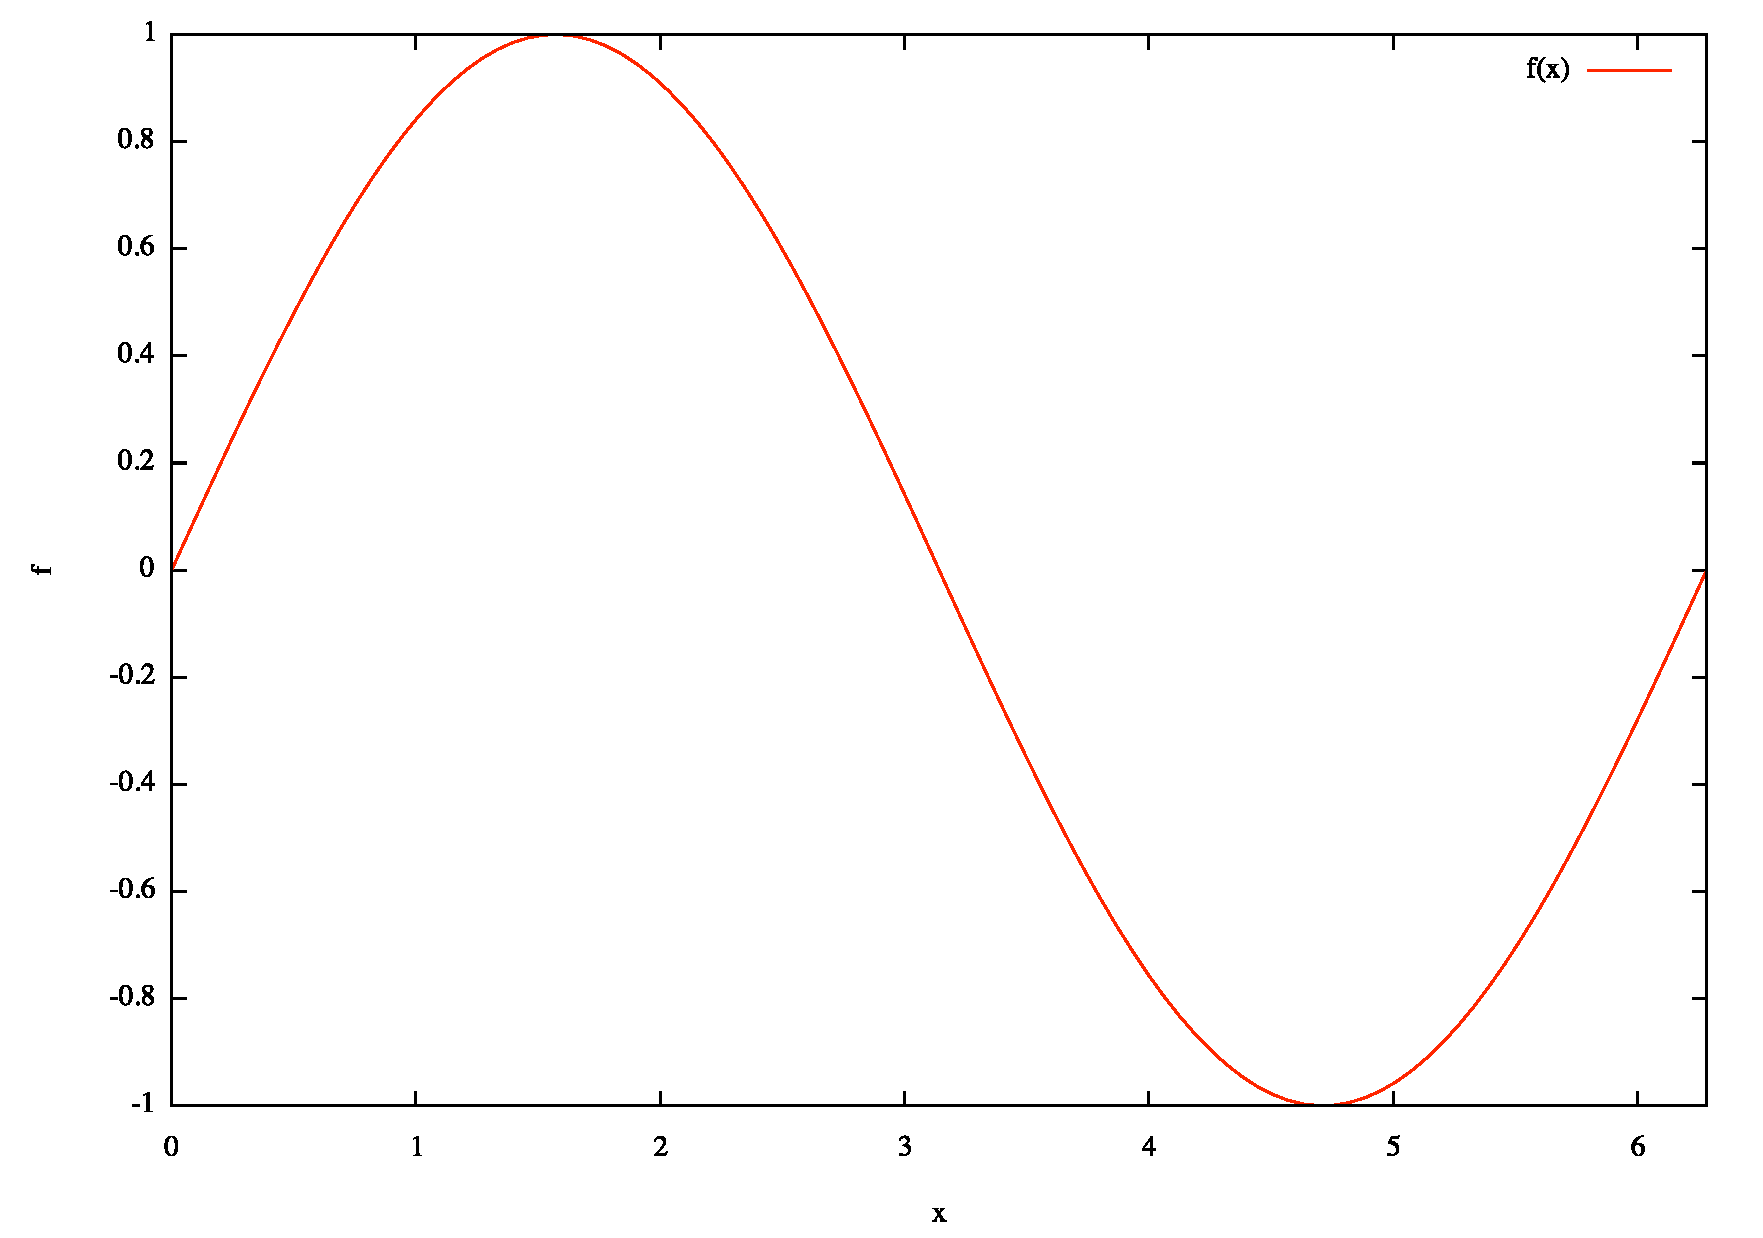
\includegraphics[width=\textwidth,keepaspectratio=true]{figure1.pdf}
\caption{Lorem ipsum dolor sit amet, consectetur adipiscing elit. In the Appendix.}\label{fig::A1}
\end{center}
\end{figure}

In ornare turpis nec nunc venenatis ac tristique felis tempor. Fusce consectetur pulvinar nisi, id tincidunt tortor ultricies non. Praesent pulvinar mollis leo, ac posuere ipsum molestie at. Suspendisse in ligula massa. Proin interdum viverra neque, et bibendum nulla lobortis at. Nunc quis mollis libero. Morbi dolor diam, tristique nec tristique in, faucibus eu metus. Donec dapibus pulvinar ante, et pretium erat molestie eu. Donec hendrerit posuere metus eu interdum. Nam neque arcu, vestibulum in aliquam in, aliquet mollis nibh. Aenean nec augue in dui bibendum ultricies nec nec odio. Cum sociis natoque penatibus et magnis dis parturient montes, nascetur ridiculus mus.

Phasellus et imperdiet justo. Pellentesque nec suscipit tortor. Aliquam ut nibh ac velit auctor congue quis at urna. Nulla convallis enim et nunc commodo varius. Sed elementum turpis ac purus sodales non luctus lacus dignissim. Cras id lorem id purus pulvinar convallis ac pulvinar elit. Morbi mattis, neque at condimentum lacinia, ipsum risus rutrum leo, non dignissim arcu eros a neque. Proin adipiscing, metus sed pulvinar suscipit, eros eros cursus velit, vel placerat turpis orci nec orci. Phasellus in dolor felis, id ultricies erat. Maecenas sollicitudin ultricies molestie.

\subsection{Vivamus}
\textcolor{red}{Vivamus dictum ligula vitae ante ornare hendrerit.} Quisque ac dolor nibh, eu ornare sem. Cras sit amet neque odio. Nulla bibendum bibendum turpis at congue. Nunc ultricies scelerisque sem, ut dapibus tellus dignissim sollicitudin. Curabitur sed sapien nibh, nec consectetur ante. Aliquam erat volutpat. Fusce tempor orci in ante venenatis nec pharetra diam aliquet. Nullam pretium elementum mauris, non commodo metus eleifend vel. Cras vel ante dolor. Suspendisse potenti. Quisque vel odio eget lorem posuere ultrices. Duis et volutpat diam. In sit amet pulvinar lacus. Vestibulum lacinia, turpis ut interdum venenatis, lorem sem eleifend diam, in hendrerit nisi tellus in lorem.
}

\typeout{**************************************************************************}
\typeout{}
\typeout{This sample file includes nomenclature (a List of Symbols). Please run:}
\typeout{     makeindex ryesample.nlo -s nomencl.ist -o ryesample.nls}
\typeout{}
\typeout{}
\typeout{This sample file includes a glossary. Please run:}
\typeout{   makeglossaries ryesample}
\typeout{}
\typeout{}
\typeout{This sample file includes an index. Please run:}
\typeout{   makeindex ryesample}
\typeout{}
\typeout{}
\typeout{This sample file includes a bibliography. Please run:}
\typeout{   bibtex ryesample}
\typeout{}
\typeout{Reprocess the document using LaTeX again, two more times to include the}
\typeout{above sections.}
\typeout{}
\typeout{**************************************************************************}


\end{document}
